\documentclass[11pt]{article}

\usepackage[a4paper,margin=1in]{geometry}
\usepackage{graphicx}
\usepackage{booktabs}
\usepackage{amsmath}
\usepackage{xcolor}
\usepackage{enumitem}
\usepackage{tikz}
\usetikzlibrary{arrows.meta,positioning,shapes.geometric}
\usepackage[colorlinks=true,linkcolor=blue!60!black,urlcolor=blue!60!black,citecolor=blue!60!black]{hyperref}
\usepackage{listings}

\definecolor{codebg}{RGB}{245,247,249}
\lstset{
  basicstyle=\ttfamily\footnotesize,
  backgroundcolor=\color{codebg},
  breaklines=true,
  frame=single,
  rulecolor=\color{gray!40},
  columns=fullflexible,
  keepspaces=true,
  showstringspaces=false,
  xleftmargin=4pt,xrightmargin=4pt,
}

\setlength{\parskip}{0.5em}
\setlength{\parindent}{0pt}

\title{\vspace{-1.5em}\textbf{AI-based Village Pond Planning System}\\[0.3em]
\large Phase 3 --- Interactive Web Application for Pond Siting,\\ Catchment Analysis and Water-Volume Estimation}
\author{Rishi Kharya (Roll No. 12341790)}
\date{\today}

\begin{document}
\maketitle
\vspace{-1.5em}

\begin{center}
\begin{tabular}{ll}
\textbf{GitHub repository:} & \url{https://github.com/krish1809/village-pond}\\
\textbf{Live front-end / API:} & \url{http://10.1.75.79:5228/} \quad(API docs: \href{http://10.1.75.79:5228/docs}{/docs})\\
\textbf{Demo video:} & \emph{[YouTube link]}\\
\end{tabular}
\end{center}

\hrule
\vspace{0.5em}

\begin{abstract}
\noindent
This phase delivers a fully working web application that lets a user select any land
area on an interactive map and, for that area, automatically suggests where a pond
could be built, delineates the catchment that would drain into it, and estimates the
volume of water it could collect. The backend fetches a real elevation model for the
selected block from OpenTopography, reconstructs the terrain, routes surface water
across it, and reasons about the result the way a person reading a topographic map
would: water runs downhill, gathers in low spots, and a pond only makes sense where
water actually collects without sitting inside a flowing watercourse. Rainfall is
obtained from the Open-Meteo historical archive and combined with the catchment and
the basin geometry to estimate collectable water and the depth required to hold a
year's runoff. All results --- suggested pond, catchment, contours and the existing
drainage network --- are overlaid on the map. Nothing is hard-coded to any one
location; the same logic runs on any region the user selects.
\end{abstract}

\section{Introduction}

Choosing a good pond site in a village normally combines three things judged by eye:
the shape of the land, how much land funnels runoff toward a point, and how much rain
falls there. Doing this manually is slow and gives no quantitative basis for sizing
the pond. This phase automates it end to end behind a single web page.

The system meets the phase requirements directly: (i) a fully working front-end;
(ii) an option to select the land area on a map; (iii) generation of results for the
selected area; (iv) results that include the \textbf{suggested pond location}, the
\textbf{catchment area} and the \textbf{expected water volume}; (v) all three overlaid
and visualised on the map; and (vi) a solution that is fast and functional within the
memory- and storage-limited systems provided. Phase 2's contour-upload route
(\texttt{POST /analyzeContour}) is retained unchanged; Phase 3 is additive.

\section{System Overview and Architecture}

The whole system runs as a \emph{single} FastAPI process: it serves both the compiled
React front-end (as static files) and the analysis API on one port. This keeps the
footprint minimal on the provided containers. The analysis reuses the Phase 2
terrain/hydrology modules unchanged --- the only difference is where the elevation
model comes from.

\begin{center}
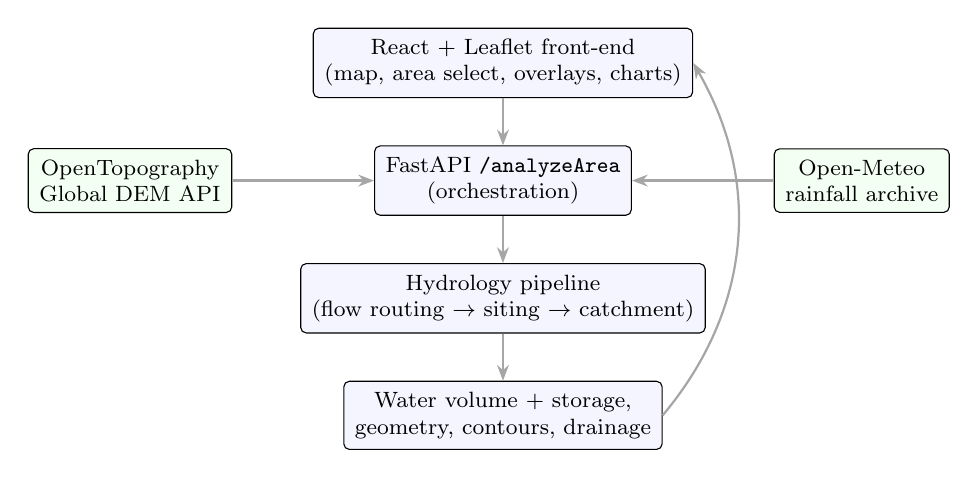
\begin{tikzpicture}[
  node distance=6mm and 10mm,
  box/.style={draw,rounded corners=2pt,align=center,inner sep=4pt,font=\footnotesize,fill=blue!4},
  ext/.style={draw,rounded corners=2pt,align=center,inner sep=4pt,font=\footnotesize,fill=green!5},
  arr/.style={-{Stealth[length=2mm]},thick,gray!70},
]
\node[box] (fe) {React + Leaflet front-end\\(map, area select, overlays, charts)};
\node[box,below=of fe] (api) {FastAPI \texttt{/analyzeArea}\\(orchestration)};
\node[ext,left=18mm of api] (dem) {OpenTopography\\Global DEM API};
\node[ext,right=18mm of api] (rain) {Open-Meteo\\rainfall archive};
\node[box,below=of api] (pipe) {Hydrology pipeline\\(flow routing $\rightarrow$ siting $\rightarrow$ catchment)};
\node[box,below=of pipe] (out) {Water volume + storage,\\geometry, contours, drainage};
\draw[arr] (fe) -- (api);
\draw[arr] (dem) -- (api);
\draw[arr] (rain) -- (api);
\draw[arr] (api) -- (pipe);
\draw[arr] (pipe) -- (out);
\draw[arr] (out.east) to[bend right=35] (fe.east);
\end{tikzpicture}
\end{center}

\textbf{Module responsibilities} (each a single, non-overlapping concern):
\texttt{elevation\_api} fetches and parses the DEM; \texttt{terrain\_grid} builds the
grid and slope; \texttt{catchment} does depression filling, flow direction, flow
accumulation and watershed delineation; \texttt{pond\_locator} scores and ranks
candidate sites; \texttt{geometry\_utils} measures areas/perimeters in metres;
\texttt{rainfall\_api} fetches rainfall; \texttt{water\_volume} computes runoff,
capacity and the storage curve; \texttt{contour\_lines} generates contours for
display; \texttt{visualization} renders the PNG figure. The route
(\texttt{analyze\_area}) only wires these together.

\section{Methodology}

\subsection{Elevation model acquisition}
For the selected bounding box, the backend requests a Digital Elevation Model (DEM)
from the \textbf{OpenTopography Global DEM API} (SRTMGL1, 30\,m). A single request
returns the whole raster for the block. The ASCII-grid (\texttt{AAIGrid}) output
format is used so it can be parsed with NumPy without any native GDAL/rasterio
dependency. The grid is oriented, cleaned of no-data values, and, if larger than a
cap, stride-downsampled to keep computation within the container's memory.

\subsection{Terrain model and slope}
The DEM is a regular grid of elevations. Local slope at each cell is computed with the
Horn (1981) finite-difference gradient:
\begin{equation}
\text{Slope} = \arctan\!\left(\sqrt{\left(\tfrac{dz}{dx}\right)^2 + \left(\tfrac{dz}{dy}\right)^2}\,\right).
\end{equation}
Cell spacing is converted from degrees to metres before slope is interpreted, since
coordinates are longitude/latitude.

\subsection{Flow routing}
Small artificial pits are removed first using the \textbf{Priority-Flood} algorithm
(Barnes et al., 2014), an $O(n\log n)$ depression fill that processes cells outward
from the boundary in elevation order. \textbf{D8 flow direction} (O'Callaghan \& Mark,
1984) then assigns each cell to its steepest-descent neighbour, where the downhill
slope toward a neighbour is
\begin{equation}
S_d = \frac{z_{\text{current}} - z_{\text{neighbour}}}{\text{distance}}.
\end{equation}
\textbf{Flow accumulation} --- the number of upstream cells draining through each cell
--- is then computed by processing the flow network in topological order. High
accumulation marks where surface water concentrates.

\subsection{Choosing where a pond makes sense}
Flow accumulation alone is not enough: a channel carries much water but is not a place
to build a pond, while a dry knoll is not either. Two terrain measures are combined.
The \textbf{Topographic Wetness Index} captures the tendency of water to gather while
accounting for slope,
\begin{equation}
\text{TWI} = \ln\!\left(\frac{\text{upslope area}}{\tan(\text{slope})}\right),
\end{equation}
and the \textbf{Topographic Position Index} captures whether a cell sits lower than its
surroundings,
\begin{equation}
\text{TPI} = z_{\text{cell}} - \overline{z}_{\text{neighbourhood}} .
\end{equation}
Both are normalised to $[0,1]$; since a \emph{lower} position is favourable, its sign
is flipped, giving the suitability score
\begin{equation}
\text{Score} = 0.5\,\text{TWI}_{\text{norm}} + 0.5\,(-\text{TPI})_{\text{norm}} .
\end{equation}
Three hard feasibility filters are then applied: cells steeper than $15^{\circ}$ are
excluded (earthen ponds are not built on steep ground); cells belonging to the
existing \textbf{drainage/channel network} (flow accumulation above the 97th
percentile, plus a small buffer) are excluded, because a pond must be fed \emph{by} a
watercourse, not sit \emph{inside} it; and a candidate whose flood-fill footprint
cannot be bounded within a growth cap is rejected, since that indicates broad
floodplain-like ground rather than a containable basin. Candidates are then chosen
greedily with a minimum-separation radius so the top sites are genuinely distinct
regions.

\subsection{Catchment delineation}
For each selected site the \textbf{catchment} (watershed) is traced by walking the
D8 flow network \emph{backwards} from the site: a neighbouring cell is included
whenever its flow direction points toward the current cell, continuing until no more
upstream contributors are found. On flat terrain the resulting watershed can be
several disconnected pieces; all pieces are retained.

\subsection{Metric geometry}
The cell masks are converted into polygons by unioning the exact cells (not an
approximating hull, which was found to overestimate area). Because longitude/latitude
are unsuitable for measuring area, polygons are projected into the appropriate
\textbf{UTM zone} --- selected automatically from the block's location --- so area and
perimeter are computed in metres. Boundaries drawn on the map are additionally
smoothed for display only; the reported areas are always measured on the exact
polygons.

\subsection{Rainfall}
Mean annual rainfall is obtained from the \textbf{Open-Meteo historical archive},
averaged over the last several complete years of daily precipitation for the block's
centre. Every call has a timeout and, if the service is unreachable, the system falls
back to a documented default annual rainfall so a volume is always produced; the
response marks which source was used.

\subsection{Water volume and storage}
Two independent limits are computed. The annual runoff the catchment delivers uses a
Rational-method estimate,
\begin{equation}
V_{\text{runoff}} = C \cdot P \cdot A_{\text{catchment}} \quad (\text{m}^3/\text{yr}),
\end{equation}
where $P$ is mean annual rainfall (m/yr), $A_{\text{catchment}}$ is the catchment area
(m$^2$) and $C$ is a runoff coefficient (default $0.3$, adjustable). The basin's
storage capacity is measured directly from the DEM over the pond footprint,
\begin{equation}
V_{\text{capacity}} = \sum_{\text{cells}} (w - z_i)\cdot A_{\text{cell}},
\end{equation}
where $w$ is the water-surface level. The realistically collectable volume is bounded
by both --- the catchment cannot deliver more, and the basin cannot hold more:
\begin{equation}
V_{\text{collectable}} = \min\!\left(V_{\text{runoff}},\, V_{\text{capacity}}\right).
\end{equation}
Finally, a stage--area--volume (\textbf{storage curve}) is built by flooding the basin
at increasing depths (bounded to the catchment), and the \textbf{required depth} ---
the depth at which the stored volume reaches one year's runoff --- is reported.

\section{Front-end}

The front-end is a React + Leaflet single-page application. The user can (i) search a
village/town/city by name (OpenStreetMap geocoding) and fly the map there; (ii) select
the land area either by ``Use current map view'' or by clicking two corners of a
rectangle; and (iii) run the analysis. Results are drawn on the map: the DEM's
elevation \textbf{contours}, the existing \textbf{drainage network} (blue), each
ranked \textbf{pond footprint} (filled region, labelled with its area), its
\textbf{catchment} (dashed outline) and a marker at the suggested \textbf{pond
location}. A side panel shows, per site, the catchment area, pond footprint, annual
runoff, basin capacity, collectable volume, required depth and a storage-curve chart,
plus a monthly rainfall chart for the area. Results can be downloaded as a rendered
\textbf{PNG}, as \textbf{GeoJSON} (ponds, catchments and drainage, for GIS tools) and
as the full \textbf{JSON} response. A plain OpenStreetMap base map is used, with Esri
satellite imagery available as a toggle.

\section{API Documentation}

\textbf{Endpoint.} \texttt{POST /analyzeArea}

\textbf{Request body (JSON).}
\begin{lstlisting}
{ "bbox": [min_lon, min_lat, max_lon, max_lat],
  "num_candidates": 3,          // 1-10, optional (default 3)
  "runoff_coefficient": 0.3 }   // optional (default 0.3)
\end{lstlisting}
A query parameter \texttt{format=image} returns a rendered PNG of the same result
instead of JSON.

\textbf{Response (\texttt{format=json}).} An object containing:
\begin{itemize}[nosep,leftmargin=1.4em]
  \item \texttt{candidates} --- ranked list; each has \texttt{location} (lat, lon,
  elevation, slope), \texttt{pond\_footprint} (area, perimeter, GeoJSON boundary,
  assumed depth), \texttt{catchment} (area, perimeter, GeoJSON boundary),
  \texttt{suitability} (the scoring factors), \texttt{water\_volume} (annual runoff,
  storage capacity, collectable volume, limiting factor) and \texttt{storage}
  (required depth, stage--area--volume curve).
  \item \texttt{contours} --- elevation contour lines generated from the DEM.
  \item \texttt{drainage} --- GeoJSON of the existing stream/channel network.
  \item \texttt{rainfall} --- mean annual rainfall, source and monthly climatology.
  \item \texttt{area\_summary} --- bbox, grid resolution, elevation range, DEM source.
  \item \texttt{metadata} --- a step-by-step processing log and total time.
\end{itemize}

\textbf{Error responses.} \texttt{422} --- the selected area is malformed, too large
or too small, or has no feasible pond site; \texttt{502} --- the DEM service could not
be reached; \texttt{500} --- an unexpected processing error (with the failing stage).
Full interactive documentation is auto-generated at \href{http://10.1.75.79:5228/docs}{/docs}.

\section{Results and Demonstration}

Figure~\ref{fig:sample} shows the system run on the provided sample region (near
Raipur, Chhattisgarh), the same terrain used in Phase 2. The 30\,m DEM
(elevation 266--298\,m) reproduces the known landscape: the diagonal blue band is the
main stream valley, with tributary channels branching from it. All three suggested
ponds are placed on drainable ground \emph{away} from the blue drainage network,
confirming the channel-exclusion logic. Table~\ref{tab:results} lists the numbers.

\begin{figure}[h]
\centering
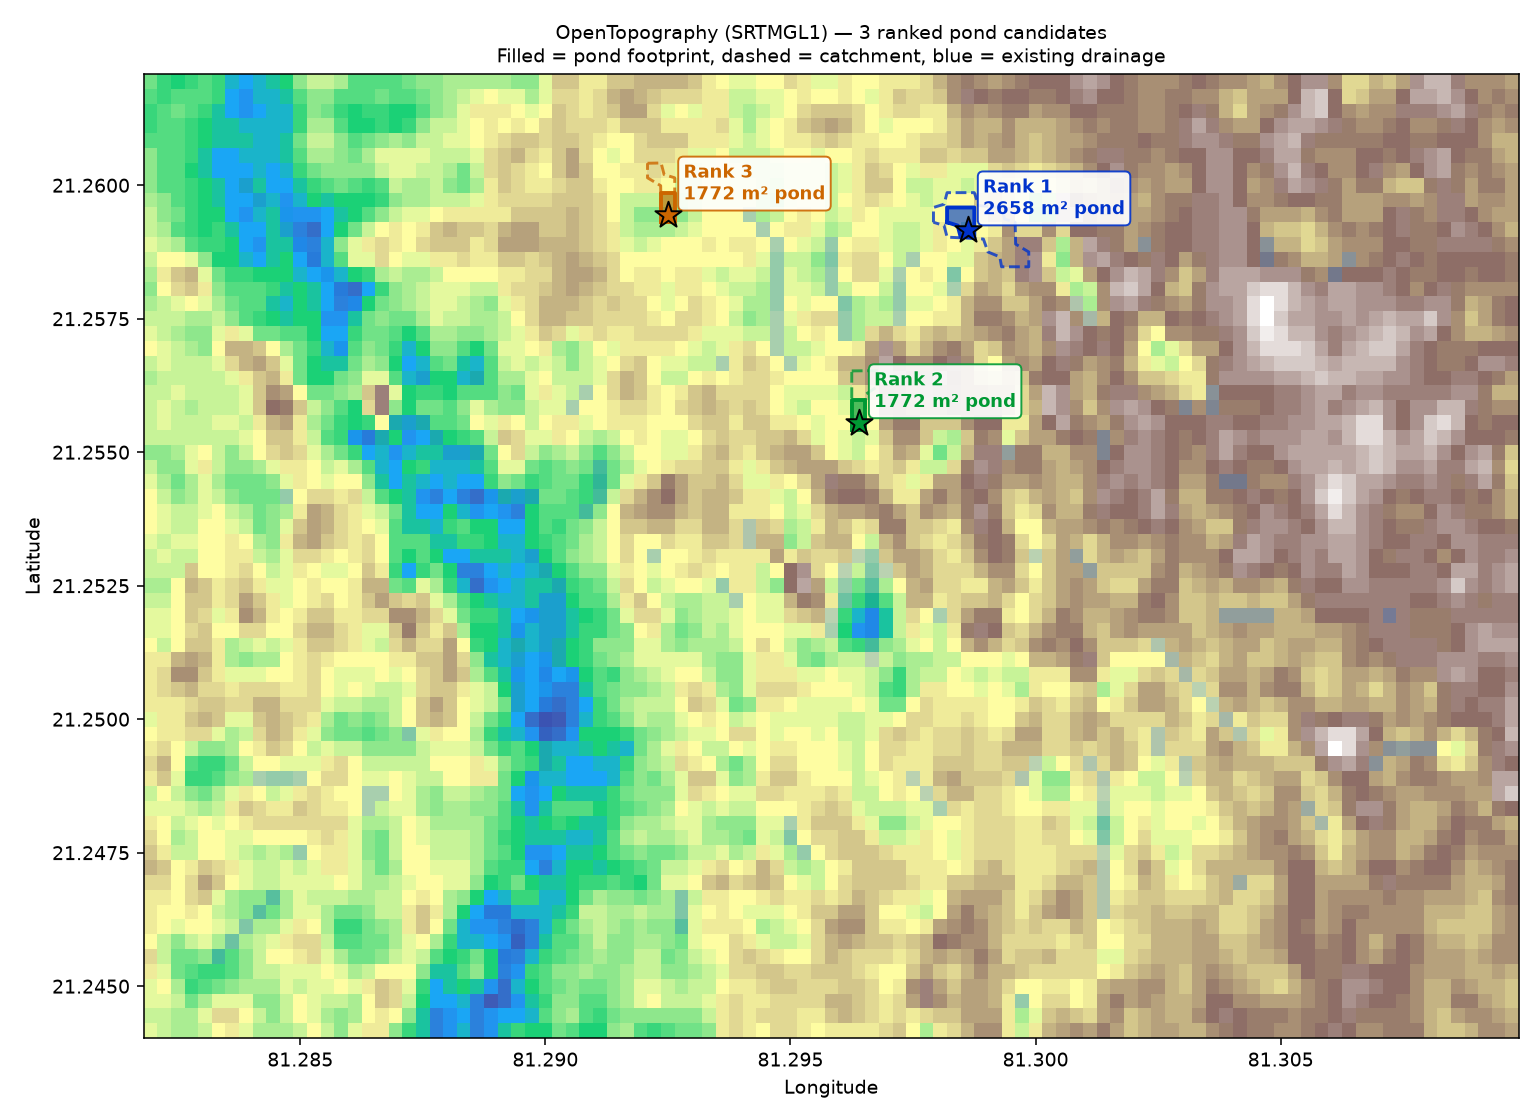
\includegraphics[width=0.95\linewidth]{figures/sample_analysis.png}
\caption{Analysis of the sample region. Terrain shading is the DEM; blue is the
existing drainage network; filled shapes are the suggested pond footprints and dashed
outlines their catchments. The ponds are correctly kept off the watercourses.}
\label{fig:sample}
\end{figure}

\begin{table}[h]
\centering
\caption{Ranked pond candidates for the sample region (grid $65\times101$,
runoff coefficient $C=0.3$). Catchment area is always $\geq$ pond footprint, as
expected.}
\label{tab:results}
\small
\begin{tabular}{clrrrrr}
\toprule
Rank & Location (lat, lon) & Catchment & Pond & Annual & Collectable & Req.\\
     &                     & (m$^2$)   & (m$^2$)& runoff (m$^3$) & (m$^3$/yr) & depth (m)\\
\midrule
1 & 21.2592, 81.2986 & 6\,202 & 2\,658 & 2\,047 & 1\,901 & 2.5\\
2 & 21.2556, 81.2964 & 2\,658 & 1\,772 & 877   & 877   & 1.0\\
3 & 21.2594, 81.2925 & 2\,658 & 1\,772 & 877   & 877   & 1.0\\
\bottomrule
\end{tabular}
\end{table}

The relationship between the quantities is internally consistent: the catchment
(water source) is always at least as large as the pond footprint (where water
collects), and the collectable volume is the smaller of what the catchment delivers
and what the basin can hold. At this DEM resolution (30\,m) over gently sloping ground
the catchments are modest; on terrain with stronger relief the same pipeline produces
correspondingly larger catchments and volumes. The end-to-end analysis, including the
live DEM fetch, completes in roughly 12 seconds and is cached thereafter.

\section{Deployment, Performance and Scaling}

The application is deployed on the provided university server and reachable at
\url{http://10.1.75.79:5228/}. The React app is built and served as static files by
the same FastAPI process, so the entire system is one process behind one URL, started
detached (\texttt{nohup}) on the container's internal port 5000 (forwarded to the
external 5228). Dependencies are installed into the pre-existing environment rather
than a duplicate virtual environment, to respect the container's small storage.

The provided containers are constrained (memory limit 512\,MB). The design stays
within this: the server's resident memory is about 160\,MB; matplotlib is imported
lazily so it is only loaded when a PNG is actually requested; the analysis grid is
capped and downsampled when necessary; and each DEM fetch and rainfall lookup is
cached in memory (keyed by area), so re-analysing the same or an adjacent block is
instant and makes no repeat external calls. Oversized area selections are rejected up
front with a clear message rather than being allowed to fan out into an expensive
request. The single-process, dependency-light design means the same build can run on
any of the four provided systems without modification.

The backend is covered by 71 automated tests (parser, terrain grid, flow/catchment,
pond locator, geometry, elevation parsing, rainfall, water volume and the image
format), all passing.

\section{Use of AI Tools}

In line with the course's LLM-usage policy, Claude (Anthropic) was used as a coding
and debugging assistant during development: to draft initial implementations of
individual modules, to explain the underlying terrain-analysis algorithms, and to help
diagnose real issues found during testing --- for example, correcting a case where the
pond footprint could exceed its catchment (resolved by clipping the footprint to the
catchment), and improving the drainage visualisation. All technical content and
implementation decisions were reviewed and are understood by the author, including the
formulas and design trade-offs described in Section~3.

\section{Conclusion}

This phase delivers a working, deployed web application that turns a user-selected map
region into concrete, ranked pond recommendations with real catchment areas and
water-volume estimates, all visualised on the map. It fetches genuine elevation and
rainfall data for the chosen area, applies a transparent and explainable hydrological
pipeline, and correctly keeps suggested ponds out of existing watercourses --- while
running comfortably within the memory and storage limits of the provided systems.

\end{document}
